\documentclass{beamer}
\usepackage{graphics}
%\usepackage[latin1]{inputenc}
\usetheme{CambridgeUS}
\title[Research articles]{Inverse methods: Hybrid Data Assimilation}
\author{Ksenia Kozhanova, Maxime Mazouth--Laurol, Michi Rakotonarivo}
\institute{Grenoble INP, MSIAM 2}
\date{January, 2018}
\begin{document}

\begin{frame}
\titlepage
\end{frame}


\begin{frame}
	\frametitle{Introduction}
	
	\begin{itemize}
		\item Hybrid techniques use the combination of several data assimilation methods
		\item Advantage fo using the benefits of several methods
		\item Better results and/or smaller computational cost
		\item Easier implementation
	\end{itemize}
\end{frame}

\begin{frame}
\frametitle{Variational Methods}

\begin{definition}
	\textbf{Data assimilation} (or data analysis) is the process by which observations of the actual system are incorporated into the model state of a numerical model of that system
\end{definition}


\begin{itemize}
	\item $\mathbf{w}$ is a state vector, $M$ is a model, $\mathbf {M} = \mathbf {M}(t_{i}, t_{i-1})$ is a linear operator related to $\delta \mathbf {w(t_{i-1})}$ and $M(t_{i},t_{i-1})$ is a non-linear model operator related to $\mathbf {w(t_{i-1})}$
	\item $ \mathbf{w} = \mathbf {w^{b}}+\delta \mathbf {w}$
	\item $\mathbf {w}(t_{i})=M(t_{i},t_{i-1})[\mathbf {w}(t_{i-1})]$
\end{itemize}
\end{frame}


\begin{frame}
	\frametitle{Variational Methods}
	
	\begin{itemize}
		\item $\mathbf {w}(t_{i}) \approx M(t_{i},t_{i-1})[\mathbf {w}^{b}(t_{i-1})] + \mathbf {M}(t_{i},t_{i-1})\delta \mathbf {w}(t_{i-1})$
		\item $\delta \mathbf {w}(t_{i}) = \mathbf {M}(t_{i},t_{i-1})\delta \mathbf {w}(t_{i-1})$
	
		\item $J(\delta \mathbf {w}) = \frac{1}{2} \delta \mathbf {w}^{T} \mathbf {B}^{-1} \delta \mathbf {w} + \frac{1}{2} \sum_{i=0}^{n}(\mathbf {G}_{i} \delta \mathbf {w} - \mathbf {d}_{i})^{T}\mathbf {R}_{i}^{-1}(\mathbf {G}_{i} \delta \mathbf {w} - \mathbf {d}_{i})$
		where $\mathbf {B}$ and $\mathbf {R}_{i}$ are matrices with covariance estimates of background and observation error, $G_{i} = H_{i}M(t_{i},t_{0})$ being a generalized observation operator, $\mathbf {G}_{i} = \mathbf {H}_{i}\mathbf {M}(t_{i},t_{0})$ being a linear observation operator
	\end{itemize}
\end{frame}


\begin{frame}
	\frametitle{4DVAR vs 3DVAR}
	\begin{itemize}
		\item The difference comes from the choice of $\mathbf{M}$ to obtain linearised observation operator $\mathbf {G}_{i}$
		\item 3DVAR: $\mathbf {M} = \mathbf {I}$, where $\mathbf {I}$
		\item 4DVAR: $\mathbf {M} \approx (\partial M/\partial \mathbf {w})|_{w-w^{b}}$
	\end{itemize}
\end{frame}


\begin{frame}
	\frametitle{Kalman theory}
	
	\begin{definition}
		\textbf{Kalman filter} The Kalman Filter is a sequential filter method, which
		means that the model is integrated forward in time and,
		whenever measurements are available, these are used to
		reinitialize the model before the integration continues ( Evensen 2003)
	\end{definition}
	
	\begin{itemize}
		\item Analysis equation $\psi ^{a} = \psi ^{f} + \textbf{P} ^{f}\textbf{H} ^{T}(\textbf{HP} ^{f}\textbf{H} ^{T}+\textbf{R}) ^{-1}(\textbf{d-H}\psi) ^{f}$
		\item $\textbf{P}^{a} = \textbf{P}^{f} - \textbf{P}^{f}\textbf{H}^{T}(\textbf{HP}^{f}\textbf{H}^{T}+\textbf{R})^{-1}\textbf{HP}^{f} $ 
		\item where  $\textbf{P}^{.}$ is the covariance for the model forecast/analysis,  $\textbf{R}$ is the covariance for the model measurements, $\textbf{H}$ is the measurement operator
		
	    \item Error covariance $\textbf{P}_{k+1}=\textbf{F}\textbf{P}_{k}\textbf{F}^{T}+\textbf{Q}$
	    \begin{itemize}
	    	\item Traditional Kalman filter: linear model $\psi_{k+1}=\textbf{F}\psi{k}$
	    	\item Extended Kalman filter: non-linear model
	    	$\psi_{k+1}=\textbf{f}(\psi_{k})$
	    	
	    \end{itemize}
	\end{itemize}
\end{frame}


\begin{frame}
	\frametitle{Ensemble Kalman filter}
	
	\begin{definition}
		\textbf{Ensemble forecasting} is the process where multiple, individual numerical forecasts
		are generated from different sets of initial conditions
		and/or different numerical model configurations (Leith 1974)
	\end{definition}
	\begin{itemize}
		
		\item analysis equation $\psi ^{a} _{j}= \psi ^{f}_{j} + \textbf{P} _{e} ^{f}\textbf{H} ^{T}(\textbf{HP}_{e} ^{f}\textbf{H} ^{T}+\textbf{R}_{e}) ^{-1}(\textbf{d}_{j}-\textbf{H}\psi ^{f}_{j})$
		
		\item error covariance $\textbf{P}_{e}^{a} = \overline {(\psi^{a} - \overline{\psi^{a}})(\psi^{a} - \overline{\psi^{a}})^{T}} =  (\textbf{I}-\textbf{K}_{e}\textbf{H})\textbf{P}_{e}^{f}$, 
		where $\textbf{K}_{e}$ is Kalman gain
		\item if we have infinite number of ensembles, we have traditional Kalman filter

	\end{itemize}
\end{frame}

\begin{frame}
	\frametitle{Hybrid methods}

	\begin{itemize}
		
		\item En3DVAR covariance matrix: $\textbf{P}^{b}_{i} = (n-2)^{-1} \sum_{j=1, j \ne i}^{n}(\textbf{x}_{j}^{b} - \overline{\textbf{x}}_{i}^{b})(\textbf{x}_{j}^{b} - \overline{\textbf{x}}_{i}^{b})^{T}$
		
		\item En4DVAR
		\begin{itemize}
			\item 4DVAR cost function $J(\textbf{w}) = \frac{1}{2} \textbf{w}^{T}\textbf{w} + \frac{1}{2}(\textbf{H}\textbf{X}'_{b}\textbf{w}+\textbf{d})^{T}\textbf{O}^{-1}(\textbf{H}\textbf{X}'_{b}\textbf{w}+\textbf{d})$
			\item En4DVAR cost function $J(\textbf{w}) = \frac{1}{2} \textbf{w}^{T}\textbf{w} + \frac{1}{2}\sum_{i=0}^{I}(\textbf{HM}\textbf{X}'_{b}\textbf{w} + \textbf{d}_{i})^{T}\textbf{O}^{-1}(\textbf{HMX}'_{b}\textbf{w}+\textbf{d}_{i})$
			\item background error in observation space:
			$\textbf{HMX}'_{b} \approx \frac{1}{\sqrt{N-1}}(HM\textbf{x}_{b1}-HM\overline{\textbf{x}_{b}}, HM\textbf{x}_{b2}-HM\overline{\textbf{x}_{b}},.....,HM\textbf{x}_{bN}-HM\overline{\textbf{x}_{b}} )$
			\item recomputed gradient of the cost function $\nabla _{w}J = \textbf{w} + \sum_{i=0}^{I}(\textbf{HMX}_{b}')^{T}\textbf{O}^{-1}(\textbf{HMX}_{b}'\textbf{w}+\textbf{d}_{i})$
		\end{itemize}
		
	\end{itemize}
\end{frame}

\section{Motivation}
\subsection{Initialization}
\begin{frame}
	\frametitle{Advantages of En4DVAR}
	
	\begin{itemize}
		
		\item combination of the unique benefits of each approach 
		\item relaxation of the requirement to have tangent linear model or adjoint model
		\item similar results with smaller computational cost
		\item appropriate data assimilation method due to the non-sequential nature
		
	\end{itemize}
\end{frame}


%----------------------Michi Part -----------------------
%-----------------------------------------
\begin{frame}{Hybrid Variational}
    Combinaison of :
    \begin{itemize}
        \item  Extended Kalman Filter 
        \item  3D-Var
    \end{itemize}
\end{frame}
%-----------------------------------------
\begin{frame}{Extended Kalman Filter}
Non-linear model
    \begin{itemize}
        \item State Forecast 
        \begin{equation}
            w_{k+1}^f = \tilde{f} (w_k^a, p_k^a)
            \label{EKFfor}
            \end{equation}
        \item  Error covariance forecast
        \begin{equation}
        P_{k+1}^f = F_k P_k^a F_k^T
        \label{CovEKF}
        \end{equation}
    where 
            \begin{equation}
            F_k = \big|_{w_k^a} \frac{\partial \tilde{f} }{ \partial w } = 
            \begin{pmatrix}
            \frac{\partial f(z,p)}{\partial w } & \frac{\partial f(z,p)}{ \partial p}\\
            0 & I 
            \end{pmatrix}  \big|_{{z_k^a},{ p_k^a}}
            \label{EKFF}
            \end{equation}
    \end{itemize}
\end{frame}
%-----------------------------------------

\begin{frame}{Extended Kalman Filter}
    \begin{itemize}
        \item Gain Matrix 
        \begin{equation}
        K_{k+1} = P_{k+1}^f H_{k+1}^T (H_{k+1} P_{k+1}^f H_{k+1}^T + R_{k+1}) ^{-1}
        \end{equation}
        where  $H_k = \big|_{w_k^a} \frac{\partial \tilde{h_k} }{ \partial w } = 
        \begin{pmatrix}
        \frac{\partial h_k(z,p)}{\partial w } & \frac{\partial h_k(z,p)}{ \partial p}\\
        0 & I 
        \end{pmatrix}  \big|_{{z_k^a},{ p_k^a}}$
        
        \item Analysis
        \begin{equation}
        w_{k+1}^a = w_{k+1}^f + K_{k+1} (y_{k+1} - H_{k+1} w_{k+1}^f)
        \end{equation}


        \item the analysis error covariance :
        \begin{equation}
            P_{k+1}^a = (I - K_{k+1} H_{k+1} ) P_{k+1}^f
        \end{equation}
    \end{itemize}
\end{frame}
%-----------------------------------------
\begin{frame}{3D-Var}
Goal:  
\begin{itemize}
    \item minimizes a cost function $J$  
    \item Find The optimal state $w^a = \underset{w} {min} J(w)$ 
\end{itemize}
    J measures the misfit between the model state $w_k$ and the background state $w_a^b$ and the observation $y_k$. \\ 
~~\\
    
Approaching: 
\begin{itemize}
        \item Cost function $J$
        \begin{equation}
        J(w_k) = (w_k - w_k^b)^T B_k^{-1} (w_k - w_k^b) + (y_k - \tilde h_k (w_k)) ^T R_k^{-1} (y_k - \tilde h (w_k)) 
        \label{costFunc}
        \end{equation}
        $B_k$ and $R_k$ are the covariance matrices of the background and observation errors
\end{itemize}

\end{frame}

%-----------------------------------------
\begin{frame}{3D-Var}
\begin{itemize}
    \item Gain Matrix 
        \begin{equation}
        K_k =  B_k \tilde H_k^T(  \tilde H_k B_k \tilde H_k^T + R_k)^{-1}
        \label{matrixGain3D}
        \end{equation}
    $\tilde H$ is the Jacobian of the observation $\tilde h_k$ evaluated at the background state $w_k^b$
    \item Analysis solution 
        \begin{equation}
        w_k^a = w_k^b + K_k (y_k - \tilde H w_k^b)
        \label{sol3D}
        \end{equation}
\end{itemize}
\end{frame}
%-----------------------------------------
\begin{frame}{Principe of Hybrid Variational}
\begin{itemize}
    \item Forecast error covariance matrix  (\ref{CovEKF}) 
        \begin{equation}
            P_k^f = 
        \begin{pmatrix}
        P_{xx_k}^f  & P_{xp_k}^f \\
        (P_{xx_k}^f)^T &  P_{pp_k}^f 
        \end{pmatrix}  
        \end{equation}
        $P_{xx_k}^f $  and $P_{pp_k}^f $ are the forecast covariance matrix \\
        $P_{xp_k}^f $ is the covariance matrix for the cross relation between the forecast errors in the state and the parameter vectors \\
        
    \item Error covariance forecast (\ref{CovEKF}) 
        \begin{equation}
        P_{k+1}^f =  
        \begin{pmatrix}
        M_k & N_k \\
        0  & I
        \end{pmatrix}
        \begin{pmatrix}
        P_{xx_k}^a & P_{xp_k}^a \\
        (P_{xx_k}^a)^T &  P_{pp_k}^a
        \end{pmatrix}
        \begin{pmatrix}
        M_k^T & 0 \\
         N_k^T & I
        \end{pmatrix}
        \end{equation}
        $M_k = \frac{\partial f(x,p) }{ \partial z} \big|_{x_k^a, p_k^a} $ and $N_k = \frac{\partial f(x,p)}{  \partial p } \big|_{x_k^a, p_k^a}$,
\end{itemize}
\end{frame}
%-----------------------------------------

\begin{frame}{Principe of Hybrid Variational}
$P_{xx_k}^f =  B_{xx}$ ; $P_{pp_k}^f = B_{pp}$  \\
\begin{itemize}
            \item Forecast error covariance simplified
                \begin{equation}
                B_{k+1} = 
                \begin{pmatrix}
                B_{xx} & N_k B_{pp} \\
                 B_{pp}N_k^T & B_{pp}
                \end{pmatrix} 
                \label{CovHyb}
                \end{equation}
\end{itemize}
\end{frame}

%-----------------------------------------
\begin{frame}{Principe of Hybrid Variational}

Analysis step : founding found by substituting the matrix (\ref{CovHyb}) into the 3D Var cost function (\ref{costFunc}) and minimizing

\begin{itemize}
            \item The gain matrix (\ref{matrixGain3D}) can now written as 
            \begin{equation}
            K_k   =   B_k \tilde H_k^T(  \tilde H_k B_k \tilde H_k^T + R_k)^{-1} = \begin{pmatrix}
            K_{x_k} \\
            K_{p_k} 
            \end{pmatrix} 
            \label{GainHyb}
            \end{equation}
    \item The state and parameter analysis (\ref{sol3D}) are given by 
        \begin{equation}
            x_k^a = x_k^b + K_{x_k} (y_k -  Hx_k^b) 
        \end{equation}
        \begin{equation}
            p_k^a = p_k^b + K_{p_k} (y_k -  Hx_k^b)
        \end{equation}
    \item Then the gain matrices (\ref{GainHyb}) is expressed as 
        \begin{equation}
        K_{x_k} = B_{xx} H^T ( HB_{xx} H^T + R_k)^{-1}
        \end{equation}
        \begin{equation}
        K_{p_k} = B_{pp} N_{k-1}^T ( HB_{xx} H^T + R_k)^{-1}
        \end{equation}

\end{itemize}
\end{frame}
%-----------------------------------------
\begin{frame}{Application of Hybrid Variational}
Linear Advection : transport of a substance by bulk motion \\

\begin{itemize}
    \item 1D linear  Model : a is the advection velocity
\begin{equation}
\frac{\partial(u)}{\partial t} + a \frac{\partial u}{ \partial x} = 0  
\label{advEq}
\end{equation}

\begin{center}
   $u(x,0) = u_0(x)  , -\infty < x < \infty$
\end{center}

The solution of (\ref{advEq}) is simply 
\begin{equation}
u(x,t) = u(x_0,0) = u_0(x-at)
\label{solAdv}
\end{equation}
\begin{center}
    $x_0 = x(0)$ and $x(t) = x_0 + at$
\end{center}
\end{itemize}
\end{frame}
%---------------------------------------------------
\begin{frame}{Application of Hybrid Variational}
\begin{itemize}
    \item Forecast model :using upwind scheme
            \begin{equation}
            u_{k+1} = A  u_k 
            \label{forecastAdv}
            \end{equation}
            where 
            \[A = 
            \begin{pmatrix}
            (1-a\mu)  & 0&   &  &a\mu \\
             a\mu  & (1-a\mu) & 0&  &\cdots \\
             &\ddots & \ddots &\ddots & 0 \\
             0 & \cdots & 0 & \mu a & (1-a\mu)
            \end{pmatrix}
            \]
    \item The \textbf{augmented system model} using (\ref{forecastAdv})
            \begin{equation}
            w_{k+1} = f(w_k) = 
            \begin{pmatrix}
            A(a_k) & 0\\
            0 & 1
            \end{pmatrix} 
            \begin{pmatrix}
            u_k\\
            a_k
            \end{pmatrix} 
            \label{MatrixA}
            \end{equation}
\end{itemize}
\end{frame}
%---------------------------------------------------
\begin{frame}{Application of Hybrid Variational}
    Since, we have only a single unknown parameter, the parameter $p^b$ is scalar and 
    \begin{equation}
        B_{pp} = \sigma_a^2
    \label{Bpp}
    \end{equation}
    where $\sigma_a^2$ is the error variance.
\end{frame}
%---------------------------------------------------
\begin{frame}{Application of Hybrid Variational}
\begin{figure}[h]
    \begin{center}
    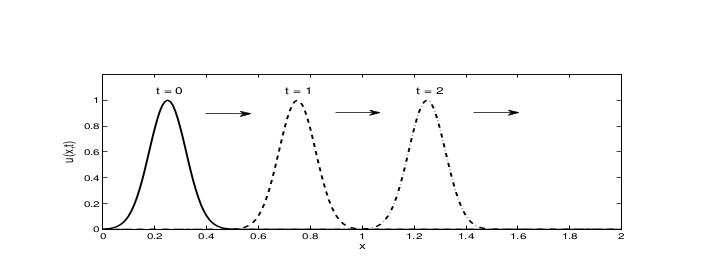
\includegraphics[width=10cm]{../Image/trueSolAdvection.png}
    \caption{Linear advection model: true solution $u(x, t)$}
    \label{trueSol}
    \end{center}
\end{figure}.
\end{frame}

%---------------------------------------------------
\begin{frame}{Application of Hybrid Variational}
\begin{figure}[h]
    \begin{center}
    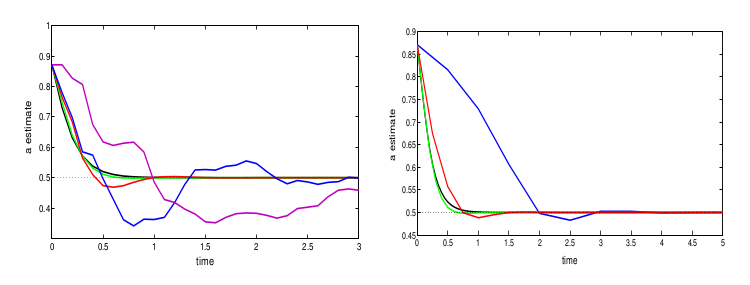
\includegraphics[width=9cm]{../Image/perfectObsAdvection.png}
    \caption{Perfect observations: parameter updates for initial estimate a = 0.87116.
(a) Varying the spatial frequency of observations (b) Varying the temporal frequency
of observations
red line - observations every$25\Delta t$; solid blue line - observations every $50\Delta t$.}
    \label{perfectObs}
    \end{center}
\end{figure}
\end{frame}

%---------------------------------------------------
\begin{frame}{Frame Title}
\begin{figure}[h]
    \begin{center}
    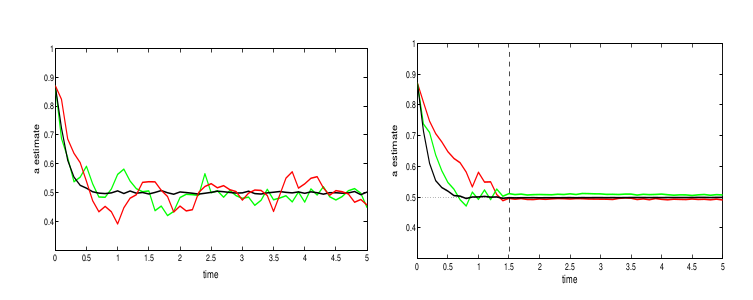
\includegraphics[width=9cm]{../Image/noisyObs.png}
    \caption{Imperfect observations: parameter updates for initial estimate $a = 0.87116$ (a) unaveraged estimates, and (b) time averaged estimates: solid black line $\sigma_0^2 = 0.001$; solid green line $\sigma_0^2 = 0.01$; solid red line $\sigma_0^2= 0.1$}
    \label{noisyObs}
    \end{center}
\end{figure}
\end{frame}
%---------------------------------------------------

\section{Iterative Ensemble Kalman Smoother}
\begin{frame}
\frametitle{Statements}
The Iterative Ensemble Kalman Smoother(IEnKS) follows the same scheme than standard Ensemble Kalman Filter :
\begin{itemize}
\item Ensemble forecast
\item Analysis
\item Posterior ensemble generation
\end{itemize}

But there are differences :
\begin{itemize}
\item  Analysis is variational
\item  Gradient of the cost function approximated using the ensemble
\end{itemize}
\end{frame}

\begin{frame}
\frametitle{Algorithm}
\begin{itemize}
\item $L$ : size of the Data Assimilation Window(DAW)
\item $S$ : number of forecast steps
\end{itemize}
\begin{center}
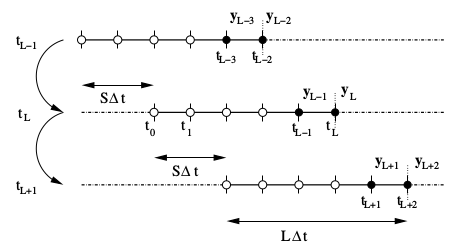
\includegraphics[scale=0.5]{../Image/IEnKS_chaining.png} 
\end{center}
Here, $L=5$ and $S=2$.
\end{frame}


\begin{frame}
\frametitle{Data assimilation monitoring}
The defined cost function :
$$\tilde{J}(w) = \frac{1}{2}(N-1)\textbf{w}^{T}\textbf{w} + \frac{1}{2}\sum_{k=1}^{L}\beta_{k}\delta_{k}^{T}(\textbf{w})\textbf{R}_{k}^{-1}\delta_{k}(\textbf{w})$$

\begin{itemize}
\item $\{\beta_k\}_{k \in [\![1,L]\!]}$ : observation weights
\item $L$ and $S$ : Overlap between consecutive DAWs.
\end{itemize}
\end{frame}

\begin{frame}
\frametitle{Numerical experiment}
\textbf{Problem statement} \\
Twin experiments together with the following Lorenz-95 model : \\
\begin{equation*}
\frac{dx_m}{dt} = (x_{m+1}-x_{m-2})x_{m-1} - x_m + F
\end{equation*}
with $x_m, m \in [\![1,M]\!]$ a variable and F the forcing parameter. \\

\textbf{Measurement metric}
$$\operatorname{RMSE}= \sqrt{\frac{\sum_{t=1}^M (x_{m}^{a} - x_{m}^{t})^2}{M}}.$$
\end{frame}
\begin{frame}
\frametitle{Overview of the results}
\framesubtitle{Parameter F known}
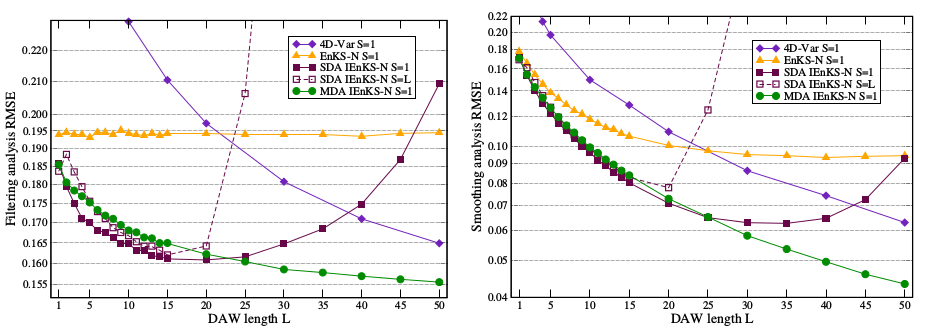
\includegraphics[width=\paperwidth,height=\paperheight]{../Image/IEnKS_weak.png}

\end{frame}

\begin{frame}
\frametitle{Augmented state principle}
\begin{itemize}
\item state vector $\textbf{x} \in \mathbb{R}^M$
\item vector of parameters $\textbf{p} \in \mathbb{R}^P$
\end{itemize}

Then, the augmented state vector is z = (x,p) 
\begin{center}
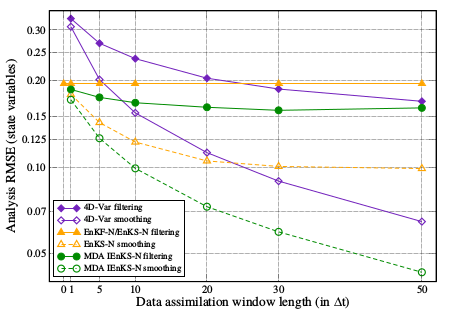
\includegraphics[scale=0.5]{../Image/IEnKS_forcing.png}
\end{center}
\end{frame}

\begin{frame}
	\frametitle{Conclusion}
	
	\begin{itemize}
		\item Four hybrid methods studied
		\item Some advantages have been discovered of using hybrid methods
		\item Understanding of the variety of data assimilation techniques involved in the hybrid methods
		
	\end{itemize}
\end{frame}

\end{document}